\documentclass{article}
\usepackage[utf8]{inputenc}
\usepackage{authblk}
\usepackage{setspace}
\usepackage[margin=1.25in]{geometry}
\usepackage{graphicx}
\graphicspath{ {./figures/} }
\usepackage{subcaption}
\usepackage{amsmath}
\usepackage{pdflscape}

%%%%%% Bibliography %%%%%%
% Replace "sample" in the \addbibresource line below with the name of your .bib file.
%\usepackage[style=authoryear,
%sorting=nyt, maxcitenames=2]{biblatex}
\usepackage[style=authoryear,sorting=nyt,maxbibnames=9,maxcitenames=2,uniquelist=false,
    backend=biber]{biblatex}
\addbibresource{reference.bib}

%%%%%% Title %%%%%%
% Full titles can be a maximum of 200 characters, including spaces. 
% Title Format: Use title case, capitalizing the first letter of each word, except for certain small words, such as articles and short prepositions
\title{Air Pollution and Heart Attacks: Transboundary Air Pollution from China to South Korea}

%%%%%% Authors %%%%%%
% Authors should be listed in order of contribution to the paper, by first name, then middle initial (if any), followed by last name.
% Authors should be listed in the order in which they will appear in the published version if the manuscript is accepted. 
% Use an asterisk (*) to identify the corresponding author, and be sure to include that person’s e-mail address. Use symbols (in this order: †, ‡, §, ||, ¶, #, ††, ‡‡, etc.) for author notes, such as present addresses, “These authors contributed equally to this work” notations, and similar information.
% You can include group authors, but please include a list of the actual authors (the group members) in the Supplementary Materials.
\author {Jung Jae Kim}

%%%%%% Affiliations %%%%%%
%\affil[1]{Department of Physics, A University, City, Country.}

%%%%%% Date %%%%%%
% Date is optional
\date{Dec 14, 2022}

%%%%%% Spacing %%%%%%
% Use paragraph spacing of 1.5 or 2 (for double spacing, use command \doublespacing)
\doublespacing

\begin{document}

\maketitle

%%%%%% Main Text %%%%%%

\section{Introduction}
Since exposure to poor ambient air quality adversely affects human health, many developed countries have tried to regulate air pollution levels. For example, U.S. Clean Air Act stated that the goal of lowering levels of air pollution was to achieve air quality standards that protect public health. Therefore, in order to identify the costs and benefits of mandating lower air pollution, the effect of air quality on observable health outcomes should be precisely estimated. However, there are challenges to estimating the causal effect, including non-random assignment and omitted variable bias. For instance, individuals who live in a region with poor air quality are likely to be in worse health status for reasons unrelated to pollution, or unobservable determinants of health (e.g. outside running) are correlated with ambient air quality. While several quasi-experimental studies try to address the challenges using a plausibly exogenous source of pollution, there are unanswered questions in this literature. First, most studies often focus on the effect of pollution on infant morality \parencite{chay2003impact,currie2005air,currie2009air}. Much less is known about short-term effects of poor air quality on health outcomes of the more general population, such as the non-elderly, non-child, adult population. Second, although the adverse effect of fine particulate matter (PM 2.5) is growing significant in Epidemiology \parencite{cox2017socioeconomic}, few studies have estimated short-term effects of PM 2.5 on health outcomes. \textcite{schlenker2016airports} have contributed to the first question by estimating the effect of exposure to carbon monoxide on general population health outcomes such as hospitalization rates for asthma, respiratory, and heart-related emergency room admissions. \textcite{deryugina2019mortality} have addressed the second issue by estimating the effect of PM 2.5 exposure on elderly mortality and medical costs. However, to the extent of my knowledge, there is no paper that answers both questions simultaneously.

I estimate the short-term effects of PM 2.5 exposure on a likelihood of having heart attacks using the rich micro-data from South Korea. I address the challenges related to non-random assignments by exploiting transboundary air pollution from China to South Korea. The air quality of South Korea is affected not only by local emissions but also by  persistent westerly winds transporting air pollutants from China, which is located west of South Korea. I use the PM 2.5 levels in Beijing, the capital of China, as an instrumental variable (IV) for the air quality in South Korea. The identifying assumption of this approach is that, after controlling location fixed effects and weather characteristics, the PM 2.5 levels in Beijing affect health outcomes in South Korea only through their influence on transboundary air pollution. By exploiting variations of pollution in China and given that persistent westerly winds travel from China to Korea, I contribute to the literature by estimating the short-term effects of PM 2.5 exposure on heart attacks of general population in South Korea.


\section{Background}
\subsection{Transboundary transport of pollutants}
South Korea was reported to have the highest average PM concentration among Organisation for Economic Co-operation and Development (OECD) countries in 2013. As a result of these environmental conditions, South Koreans' concerns about the harmful effects of exposure to PM pollution have grown. However, due to the transboundary nature of air pollution in the East Asian region, mitigating it in South Korea presents a challenging health policy issue. In fact, the majority of high PM levels in South Korea were related to pollution increases caused by wind flows from an external pollution source, such as eastern mainland China \parencite{lee2011high,lee2017estimating}.

The features of pollutants and local climatic circumstances can explain the transboundary transfer of pollutants from China to South Korea. First, due to its small size, PM 2.5 can be transported to long-range transboundary since it can stay in the atmosphere for days or even weeks \parencite{national2010global}. Significant amounts of pollutants are predominantly concentrated in eastern mainland China, and there are persistent wind flows that can transport pollutants to Korea.
According to field studies on air quality conducted through international cooperation among East Asian countries (KORUS-AQ, 2017), 52\% of Korean pollution was due to domestic factors, and 34\% was due to Chinese sources. In addition to the transported pollutants that have an impact on South Korea's PM levels, precursor particles like sulfate or nitrate are also transported, and they can produce secondary PM or gaseous pollutants (KORUS-AQ, 2017).

Second, seasonal winds in the East Asian region affect the transportation of pollutants from China. Combined with westerly winds, seasonal fluctuations in the high- and low-pressure systems in the area can either intensify or weaken the wind flows. For instance, the strongest seasonal winds that blow from China to Korea occur during the winter when high-pressure systems over northwest China combine with low-pressure systems in the Pacific Ocean. However, as high-pressure systems over the southern Pacific strengthen during the summer, the wind's velocity decreases, and its direction changes. In conclusion, except for the summer, this seasonal wind pattern enables pollutants produced from the concentrated industrial complex in the eastern area of China to be transported to regions in the East, including South Korea. In addition, it typically takes one day on average for pollutants from Beijing to reach South Korean cities \parencite{lee2011high}. By doing the wind back-trajectory analysis, the identification of transboundary sources in this paper can be more clearly understood. While local emissions are likely to be the source of the high PM 2.5 levels in Summer, the eastern area of China can be recognized as the source region for the high PM events in other seasons.

\subsection{Fine particulate matter and heart attacks}
Still working on this literature.

\section{Data}
\subsection{Pollution in South Korea}
Although the level of five major pollutants (PM10, CO, NO2, SO2, and O3) has been recorded since 2001, the level of our main interest of pollutant, PM2.5, has been observed since 2015 from Air Korea, the information center in charge of real-time ambient air pollution recordings from 505 monitors across the country. Specifically, the hourly recordings of PM2.5 are collected from Air Korea, and I mainly focus on Seoul, the capital of South Korea, and other 6 metropolitan cities because the likelihood of having heart attacks is also influenced by unobservable characteristics of patients' location, such as the intensity of locally emitted pollution. Our sample period is from January 2015 to June 2017, which is the last date when the level of PM2.5 is observed in China. Then I take a monthly average of PM2.5 from hourly recordings for each metropolitan city. 

\subsection{Pollution in China}
Given persistent westerly winds from China to Korea, the pollution levels in China's northeastern region, which has a concentrated industrial complex, are considered to be a significant location of transboundary pollutants. Although many pollution monitors are operated by the Chinese government, it is infeasible to retrieve historical data from these monitors due to access restrictions to data by the Chinese government and the possibility of non-classical measurement error caused by under-reporting or bunching at the thresholds \parencite{chen2012gaming,ghanem2014effortless}.

Therefore, similar to \textcite{jung2022transboundary}, I use the historical PM2.5 recordings from the monitor located at the U.S. embassy in Beijing, which is administered by the U.S. Department of State Air Quality Monitoring program from 2015 to June 2017. Since Beijing is not far from the Northeastern region of China, I assume that the Beijing monitor’s recordings are a credible proxy for the pollution level in Northeastern China. Again, I take a monthly average of PM2.5 from hourly recordings of Beijing. 

Figure 1 and Figure 2 present time trends in PM 2.5 air pollution in South Korea and China, respectively. They show similar trends each other, and as explained before, high pollution levels during winter in Beijing seem to affect high pollution levels in South Korea.

\begin{figure}[h]
    \centering
    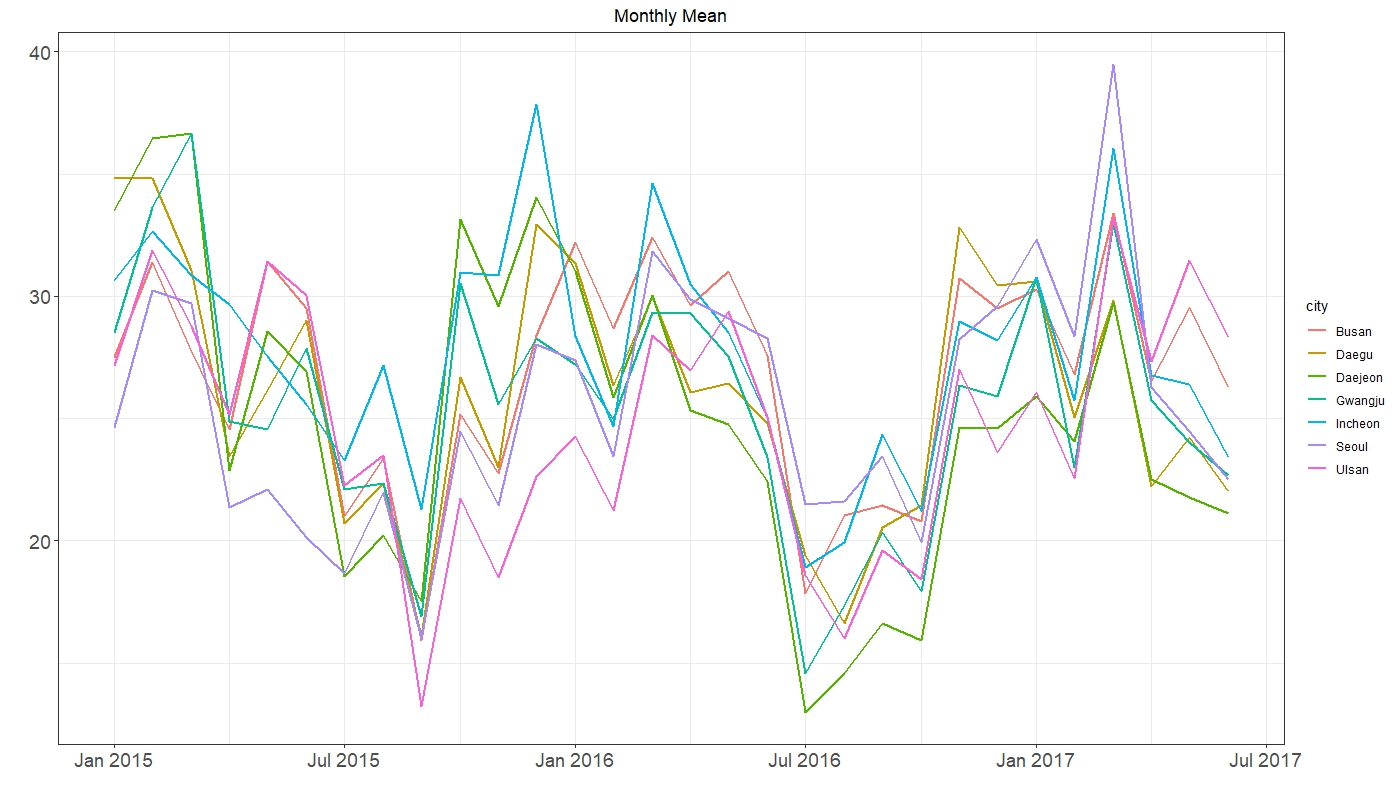
\includegraphics[width=0.8\textwidth]{figures/pm25_Korea.jpeg}
    \caption{Trends in PM 2.5 Air Pollution in Metropolitan Cities in South Korea.}
    \label{fig:1}
    \bigskip
    \bigskip
    \centering
    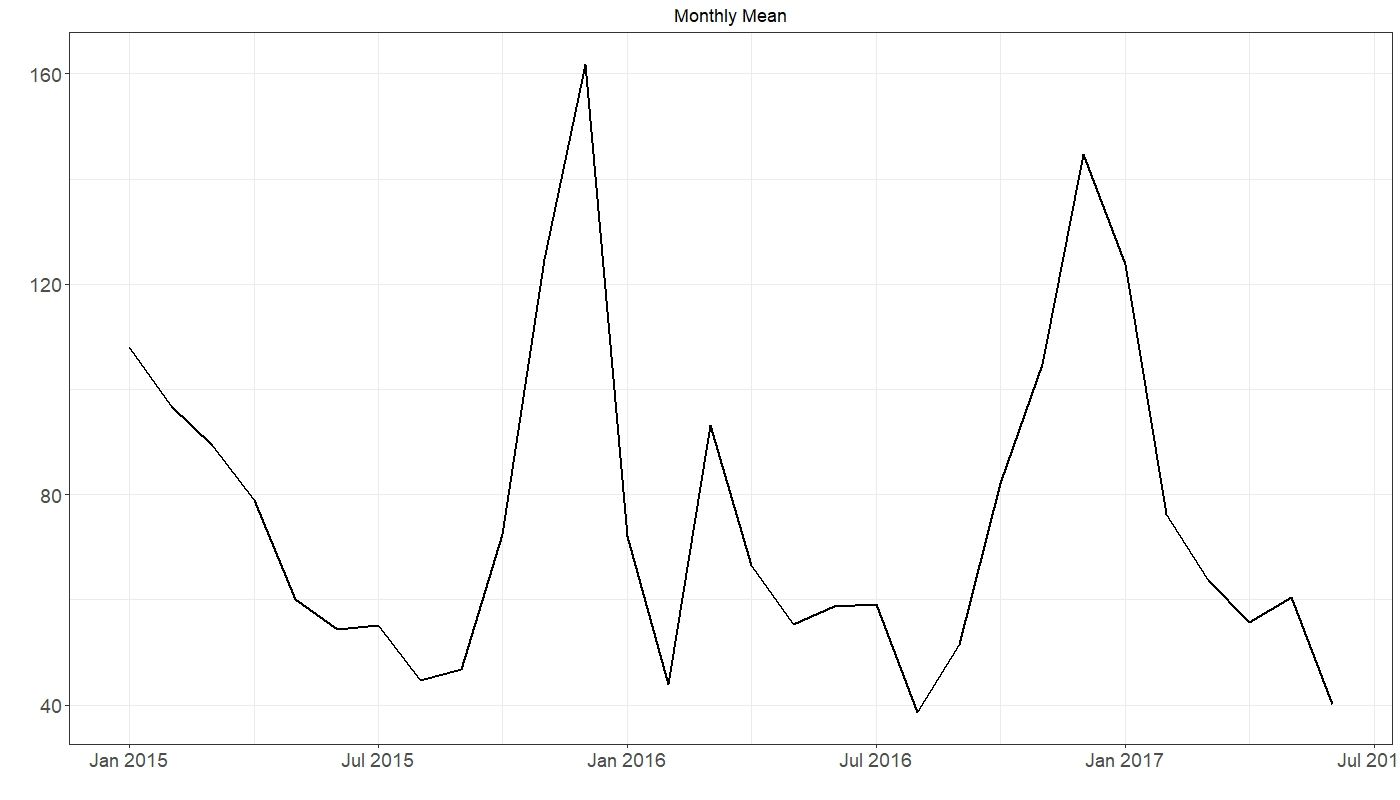
\includegraphics[width=0.8\textwidth]{figures/pm25_Beijing.jpeg}
    \caption{Trends in PM 2.5 Air Pollution in Beijing.}
    \label{fig:2}
\end{figure}


\subsection{Weather in South Korea}
Still working on this data

\subsection{Heart attacks in South Korea}
Statistics Korea has provided rich information about emergency room admissions of heart attacks. Data include the date of occurrence, causes of heart attacks, and patients' characteristics such as gender, age, and residential area. I exclude the case where the cause of heart attacks is external damage such as traffic accidents, accidental falls, stabs, burns, or suffocation. Therefore, our sample only includes heart attacks caused by diseases. Then I categorize patients' age into three groups: 'Youth' aged younger than 19, 'Adult' aged between 19 and 64, and 'Elder' aged older than 65 so that I can estimate the age-specific heterogeneous effects of PM 2.5 exposure on heart attacks. Table 1 presents summary statistics of reported heart attacks by region, year, and age group.

\section{Empirical Methodology}
This study is estimating the causal link between PM 2.5 levels and heart attacks for general population in the metropolitan cities of South Korea. I use PM 2.5 levels in Beijing as an instrumental variable for PM 2.5 levels in South Korea in the following first stage regression equation:
\begin{equation} \label{eq:1}
    \textbf{First Stage:} \; PM2.5_{ct} = \alpha_1 BeijingPM2.5_{t} + \mathbf{Z}_{ct}\Gamma + v_c + \epsilon_{ct}
\end{equation}

where $PM2.5_{ct}$ is PM 2.5 levels in a city $c$ in South Korea at time $t$, Beijing$PM2.5_{t}$ is PM 2.5 levels in Beijing, $\mathbf{Z}_{ct}$ weather controls, and $v_c$ is a city fixed-effects.

\begin{equation} \label{eq:2}
    \textbf{Second Stage:} \; Heart attacks_{ct} = \beta_1 \hat{PM2.5}_{ct} + \mathbf{Z}_{ct}\Gamma + v_c + e_{ct}
\end{equation}

where $Heart attacks_{ct}$ is the number of reported heart attacks in a city $c$ at time $t$, and $\hat{PM2.5}_{ct}$ is a fitted value from the first stage equation (1).\\\\
\textbf{Further things to do and thoughts}: I can also use other health outcome variables other than heart attacks such as infant mortality, asthma, and respiratory hospitalization rate. I might consider using a distance from Beijing to each metropolitan city in the first stage, but South Korea is a very small country. Aggregating hourly data to monthly data loses a lot of information. Should I aggregate hourly data to daily data instead? But the daily number of heart attacks reported might not be big enough. How do I incorporate seasonal variation in the model.

\newpage
\begin{landscape}
\begin{table}[b]
\caption{Summary statistics of the number of reported heart attacks.}    
\centering
\begin{tabular}{cc|cccc|cccc|cccc|cccc}
\hline
\multicolumn{2}{c}{City} & \multicolumn{4}{c}{Seoul} & \multicolumn{4}{c}{Incheon} & \multicolumn{4}{c}{Daejeon} & \multicolumn{4}{c}{Daegu} \\
Age group & Year & Mean & Std.Dev. & Min & Max & Mean & Std.Dev. & Min & Max & Mean & Std.Dev. & Min & Max & Mean & Std.Dev. & Min & Max \\
\hline
\multirow{ Adult } & 2015 & 107.25 & 9.69 & 84 & 119 & 38.17 & 7.4 & 25 & 53 & 15.83 & 4.41 & 9 & 25 & 27.5 & 7.98 & 15 & 44 \\
& 2016 & 100.33 & 10.11 & 89 & 120 & 35.83 & 8.8 & 21 & 52 & 14.58 & 3.85 & 8 & 21 & 31.75 & 7.47 & 22 & 50 \\
& 2017 & 101.58 & 17.86 & 65 & 130 & 34.83 & 8.52 & 17 & 51 & 14.92 & 3.96 & 9 & 20 & 29.33 & 5.43 & 20 & 37 \\
\hline
\multirow{ Elder } & 2015 & 209.33 & 39.72 & 153 & 283 & 61.42 & 9.65 & 44 & 81 & 29.08 & 7.44 & 18 & 42 & 54.25 & 7.97 & 45 & 70 \\
& 2016 & 191.67 & 34.64 & 141 & 253 & 55.08 & 10.74 & 35 & 66 & 25.92 & 6.83 & 9 & 34 & 50.58 & 7.39 & 40 & 64 \\
& 2017 & 191.58 & 37.09 & 127 & 263 & 58.75 & 10.15 & 43 & 80 & 25.25 & 5.99 & 15 & 35 & 56.17 & 11.38 & 36 & 79 \\
\hline
\multirow{ Youth } & 2015 & 5.17 & 1.59 & 2 & 8 & 2.22 & 0.97 & 1 & 4 & 1.5 & 0.76 & 1 & 3 & 1.73 & 0.79 & 1 & 3 \\
& 2016 & 3.45 & 1.69 & 2 & 7 & 2.22 & 1.64 & 1 & 5 & 1.43 & 0.53 & 1 & 2 & 2 & 0.87 & 1 & 3 \\
& 2017 & 3.42 & 1.51 & 1 & 6 & 1.9 & 0.99 & 1 & 4 & 1.75 & 0.5 & 1 & 2 & 1.56 & 0.53 & 1 & 2 \\
\hline
\end{tabular}
\label{tab:1}
\end{table}

\begin{table}[b]
 
\centering
\begin{tabular}{cc|cccc|cccc|cccc}
\hline
\multicolumn{2}{c}{City} & \multicolumn{4}{c}{Busan} & \multicolumn{4}{c}{Ulsan} & \multicolumn{4}{c}{Gwangju} \\
Age group & Year & Mean & Std.Dev. & Min & Max & Mean & Std.Dev. & Min & Max & Mean & Std.Dev. & Min & Max \\
\hline
\multirow{ Adult } & 2015 & 42.92 & 7.34 & 31 & 54 & 12.67 & 2.67 & 9 & 18 & 14 & 3.79 & 9 & 21 \\
& 2016 & 46.17 & 8.63 & 36 & 62 & 13 & 1.76 & 10 & 15 & 13.92 & 4.4 & 6 & 21 \\
& 2017 & 41.42 & 6.2 & 32 & 50 & 14 & 4.2 & 8 & 21 & 15.5 & 2.84 & 10 & 20 \\
\hline
\multirow{ Elder } & 2015 & 79.25 & 11.89 & 64 & 104 & 16.92 & 4.85 & 8 & 25 & 26 & 6.51 & 13 & 38 \\
& 2016 & 73.33 & 17.05 & 54 & 110 & 16.92 & 3.09 & 13 & 24 & 24.5 & 7.39 & 11 & 35 \\
& 2017 & 74.25 & 15.77 & 53 & 105 & 15.75 & 5.51 & 6 & 27 & 21.17 & 6.48 & 13 & 31 \\
\hline
\multirow{ Youth } & 2015 & 2.1 & 1.1 & 1 & 4 & 1.38 & 0.52 & 1 & 2 & 1.71 & 0.95 & & 3 \\
& 2016 & 1.67 & 0.71 & 1 & 3 & 2 & 1.22 & 1 & 4 & 1.67 & 0.71 & 1 & 3 \\
& 2017 & 2.22 & 1.09 & 1 & 4 & 1.71 & 0.76 & 1 & 3 & 1.67 & 1 & 1 & 4 \\
\hline
\end{tabular}
\label{tab:1}
\end{table}

\end{landscape}


\printbibliography

\end{document}
